% F049: native TikZ/PGFPlots, computed from the stated mathematical model.
\begin{center}
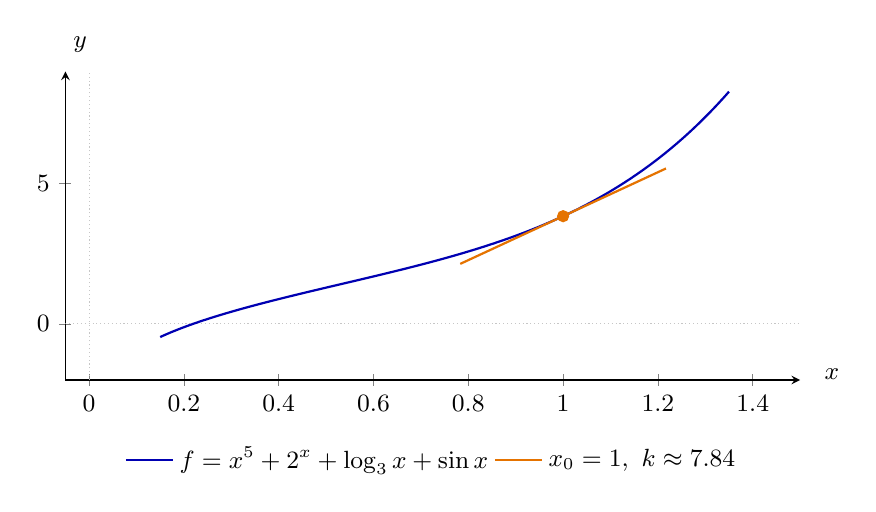
\begin{tikzpicture}[font=\small,>=stealth]
\begin{axis}[width=.90\linewidth,height=5.5cm,xmin=-0.05,xmax=1.5,ymin=-2,ymax=9,
axis lines=left,xlabel={$x$},ylabel={$y$},font=\small,
xlabel style={at={(axis description cs:1.02,.02)},anchor=west},
ylabel style={rotate=-90,at={(axis description cs:.02,1.03)},anchor=south},
legend style={at={(axis description cs:.5,-.18)},anchor=north,draw=none,fill=none,font=\small,legend columns=2},
unbounded coords=jump,clip=true,]
\addplot[gray!45,thin,densely dotted,forget plot] coordinates {(-0.05,0) (1.5,0)};
\addplot[gray!45,thin,densely dotted,forget plot] coordinates {(0,-2) (0,9)};
\addplot[blue!70!black,thick] coordinates {(0.15,-0.46774949) (0.15666667,-0.41642159) (0.16333333,-0.36672313) (0.17,-0.31852181) (0.17666667,-0.27170052) (0.18333333,-0.2261551) (0.19,-0.18179247) (0.19666667,-0.13852911) (0.20333333,-0.096289741) (0.21,-0.055006306) (0.21666667,-0.01461701) (0.22333333,0.024934416) (0.23,0.063699389) (0.23666667,0.10172502) (0.24333333,0.13905463) (0.25,0.17572813) (0.25666667,0.21178241) (0.26333333,0.24725165) (0.27,0.28216761) (0.27666667,0.31655985) (0.28333333,0.35045598) (0.29,0.38388182) (0.29666667,0.41686158) (0.30333333,0.44941802) (0.31,0.48157256) (0.31666667,0.51334544) (0.32333333,0.54475578) (0.33,0.57582173) (0.33666667,0.60656051) (0.34333333,0.6369885) (0.35,0.66712134) (0.35666667,0.69697398) (0.36333333,0.7265607) (0.37,0.75589524) (0.37666667,0.78499078) (0.38333333,0.81386001) (0.39,0.84251521) (0.39666667,0.87096821) (0.40333333,0.89923049) (0.41,0.92731318) (0.41666667,0.95522711) (0.42333333,0.98298281) (0.43,1.0105906) (0.43666667,1.0380604) (0.44333333,1.0654022) (0.45,1.0926256) (0.45666667,1.11974) (0.46333333,1.1467548) (0.47,1.1736791) (0.47666667,1.200522) (0.48333333,1.2272924) (0.49,1.2539992) (0.49666667,1.2806512) (0.50333333,1.307257) (0.51,1.3338253) (0.51666667,1.3603647) (0.52333333,1.3868838) (0.53,1.413391) (0.53666667,1.4398949) (0.54333333,1.4664039) (0.55,1.4929267) (0.55666667,1.5194716) (0.56333333,1.5460472) (0.57,1.5726621) (0.57666667,1.5993248) (0.58333333,1.626044) (0.59,1.6528282) (0.59666667,1.6796861) (0.60333333,1.7066266) (0.61,1.7336584) (0.61666667,1.7607904) (0.62333333,1.7880314) (0.63,1.8153906) (0.63666667,1.842877) (0.64333333,1.8704998) (0.65,1.8982682) (0.65666667,1.9261915) (0.66333333,1.9542793) (0.67,1.9825411) (0.67666667,2.0109864) (0.68333333,2.0396252) (0.69,2.0684671) (0.69666667,2.0975223) (0.70333333,2.1268007) (0.71,2.1563127) (0.71666667,2.1860685) (0.72333333,2.2160787) (0.73,2.2463538) (0.73666667,2.2769046) (0.74333333,2.3077419) (0.75,2.3388768) (0.75666667,2.3703203) (0.76333333,2.4020839) (0.77,2.434179) (0.77666667,2.4666171) (0.78333333,2.49941) (0.79,2.5325697) (0.79666667,2.5661081) (0.80333333,2.6000376) (0.81,2.6343705) (0.81666667,2.6691194) (0.82333333,2.704297) (0.83,2.7399163) (0.83666667,2.7759903) (0.84333333,2.8125322) (0.85,2.8495555) (0.85666667,2.8870739) (0.86333333,2.925101) (0.87,2.963651) (0.87666667,3.0027379) (0.88333333,3.0423761) (0.89,3.0825802) (0.89666667,3.1233649) (0.90333333,3.1647451) (0.91,3.2067361) (0.91666667,3.2493531) (0.92333333,3.2926117) (0.93,3.3365276) (0.93666667,3.3811168) (0.94333333,3.4263955) (0.95,3.4723799) (0.95666667,3.5190868) (0.96333333,3.5665329) (0.97,3.6147352) (0.97666667,3.6637109) (0.98333333,3.7134776) (0.99,3.7640528) (0.99666667,3.8154545) (1.0033333,3.8677009) (1.01,3.9208102) (1.0166667,3.974801) (1.0233333,4.0296923) (1.03,4.0855029) (1.0366667,4.1422522) (1.0433333,4.1999598) (1.05,4.2586454) (1.0566667,4.3183289) (1.0633333,4.3790307) (1.07,4.4407712) (1.0766667,4.5035711) (1.0833333,4.5674515) (1.09,4.6324336) (1.0966667,4.6985388) (1.1033333,4.7657889) (1.11,4.8342059) (1.1166667,4.903812) (1.1233333,4.9746298) (1.13,5.0466821) (1.1366667,5.1199917) (1.1433333,5.1945821) (1.15,5.2704769) (1.1566667,5.3476997) (1.1633333,5.4262749) (1.17,5.5062266) (1.1766667,5.5875795) (1.1833333,5.6703587) (1.19,5.7545892) (1.1966667,5.8402965) (1.2033333,5.9275064) (1.21,6.016245) (1.2166667,6.1065384) (1.2233333,6.1984134) (1.23,6.2918968) (1.2366667,6.3870158) (1.2433333,6.4837978) (1.25,6.5822707) (1.2566667,6.6824624) (1.2633333,6.7844013) (1.27,6.888116) (1.2766667,6.9936355) (1.2833333,7.100989) (1.29,7.2102061) (1.2966667,7.3213166) (1.3033333,7.4343506) (1.31,7.5493386) (1.3166667,7.6663114) (1.3233333,7.7853) (1.33,7.9063358) (1.3366667,8.0294505) (1.3433333,8.1546761) (1.35,8.282045)};
\addlegendentry{$f=x^5+2^x+\log_3x+\sin x$}
\addplot[orange!90!black,thick] coordinates {(0.783,2.1408776) (1.217,5.5420644)};
\addlegendentry{$x_0=1,\ k\approx7.84$}
\addplot[only marks,mark=*,orange!90!black,forget plot] coordinates {(1,3.841471)};

\end{axis}
\end{tikzpicture}
\par\smallskip{\small 按本题原函数绘图；切线斜率由本题的导函数计算。}
\end{center}
